\newcommand\COURSE{ciss445}
\newcommand\ASSESSMENT{q1204}
\newcommand\ASSESSMENTTYPE{Quiz}
\newcommand\POINTS{\textwhite{xxx/xxx}}

\makeatletter
\DeclareOldFontCommand{\rm}{\normalfont\rmfamily}{\mathrm}
\DeclareOldFontCommand{\sf}{\normalfont\sffamily}{\mathsf}
\DeclareOldFontCommand{\tt}{\normalfont\ttfamily}{\mathtt}
\DeclareOldFontCommand{\bf}{\normalfont\bfseries}{\mathbf}
\DeclareOldFontCommand{\it}{\normalfont\itshape}{\mathit}
\DeclareOldFontCommand{\sl}{\normalfont\slshape}{\@nomath\sl}
\DeclareOldFontCommand{\sc}{\normalfont\scshape}{\@nomath\sc}
\makeatother

\input{myquizpreamble}
\input{yliow}
\input{\COURSE}
\textwidth=6in

\renewcommand\TITLE{\ASSESSMENTTYPE \ \ASSESSMENT}

\newcommand\topmattertwo{
\topmatter
\score \\ \\
Open \texttt{main.tex} and enter answers (look for
\texttt{answercode}, \texttt{answerbox}, \texttt{answerlong}).
Turn the page for detailed instructions.
To rebuild and view pdf, in bash shell execute \texttt{make}.
To build a gzip-tar file, in bash shell execute \texttt{make s} and
you'll get \texttt{submit.tar.gz}.
}

\newcommand\tf{T or F or M}
\newcommand\answerbox[1]{\textbox{#1}}
\newcommand\codebox[1]{\begin{console}#1\end{console}}

\usepackage{pifont}
\newcommand{\cmark}{\textred{\ding{51}}}
\newcommand{\xmark}{\textred{\ding{55}}}

\newcounter{qc}
\newcommand\nextq{
%\newpage
\addtocounter{qc}{1}
Q{\theqc}.
}

\DefineVerbatimEnvironment%
 {answercode}{Verbatim}
 {frame=single,fontsize=\footnotesize}

\newenvironment{largebox}[1]{%
 \boxparone{#1}
}
{}

\usepackage{environ}
\let\oldquote=\quote
\let\endoldquote=\endquote
\let\quote\relax
\let\endquote\relax

% ADDED 2021/09/09
\renewcommand\boxpar[1]{
 \[
  \framebox[\textwidth][c] {
   \parbox[]{\dimexpr\textwidth - 0.25cm} {#1}
  }
 \]
}

\NewEnviron{answerlong}%
  {\vspace{-1mm} \global\let\tmp\BODY\aftergroup\doboxpar}

\newcommand\doboxpar{%
  \let\quote=\oldquote
  \let\endquote=\endoldquote
  \boxpar{\tmp}
}

\newenvironment{mcq}[7]%
{% begin code
#1 \dotfill{#2}
 \begin{tightlist}
 \item[(A)] #3
 \item[(B)] #4
 \item[(C)] #5
 \item[(D)] #6
 \item[(E)] #7 
 \end{tightlist}
}%
{% end code
} 

\renewcommand\EMAIL{}
\newcommand\score{%
\vspace{-0.6in}
\begin{flushright}
Score: \answerbox{\POINTS}
\end{flushright}
\vspace{-0.4in}
\hspace{0.7in}\AUTHOR
\vspace{0.2in}
}

\newcommand\blankline{\mbox{}\\ }

\newcommand\ANSWER{\textsc{Answer:}\vspace{-2mm}}

\newcommand\LATEXHELPTHREEFIVEZERO{
In the \texttt{answerlong}, you will need to enter \LaTeX\ code for
mathematical notation.
Some incomplete or wrong answers are included in the \texttt{answerlong}
so that all you need to do is to make minor modifications.
Note that \texttt{answercode} is for writing code/pseudocode and
does not require mathematical notation.

Here are some pointers on writing math \LaTeX\ code:
\begin{enumerate}[nosep]

\item For \lq\lq inline math mode", use \texttt{\$...\$}.
Example: \texttt{\$x\ =\ 42\ +\ y\$} gives you $x = 42 + y$.
(Mathematical expressions have their own spacing, special symbols,
and are in italics.)

\item For \lq\lq display math mode", use \texttt{\textbackslash[...\textbackslash]}.
Example: \texttt{\textbackslash[\ x\ =\ 42 \textbackslash]} gives you \[ x = 42 \]
(Display math mode is used for emphasis.)

\item Here's how you do fractions:
\texttt{\$\textbackslash frac\{1\}\{2\}\$} gives you $\frac{1}{2}$.

\item Here's how you do subscript:
\texttt{\$t\_\{123\}\$} gives you $t_{123}$. 

\item Here's how you do superscript:
\texttt{\$n\^{}\{123\}\$} gives you $n^{123}$.
\end{enumerate}

The above information should be enough for this quiz.
For more information on \LaTeX\, you can go to
\href{http://bit.ly/yliow0/}{my website},
click on Yes you are one of my students, scroll down to the Tutorials
section and click on latex.pdf.
}

\newcommand\LATEXHELPTHREEFIVEZEROB{
In the \texttt{answerlong}, you will need to enter \LaTeX\ code for
mathematical notation.
Some incomplete or wrong answers are included in the \texttt{answerlong}
so that all you need to do is to make minor modifications.
Note that \texttt{answercode} is for writing code/pseudocode and
does not require mathematical notation.

Here are some pointers on writing math \LaTeX\ code:
\begin{enumerate}[nosep]

\item For \lq\lq inline math mode", use \texttt{\$...\$}.
Example: \texttt{\$x\ =\ 42\ +\ y\$} gives you $x = 42 + y$.
(Mathematical expressions have their own spacing, special symbols,
and are in italics.)

\item For \lq\lq display math mode", use \texttt{\textbackslash[...\textbackslash]}.
Example: \texttt{\textbackslash[\ x\ =\ 42 \textbackslash]} gives you \[ x = 42 \]
(Display math mode is used for emphasis.)

\item Here's how you do fractions:
\texttt{\$\textbackslash frac\{1\}\{2\}\$} gives you $\frac{1}{2}$.

\item Here's how you do subscript:
\texttt{\$t\_\{123\}\$} gives you $t_{123}$. 

\item Here's how you do superscript:
  \texttt{\$n\^{}\{123\}\$} gives you $n^{123}$.
  
\item Here's how you do log:
  \texttt{\$\textbackslash lg n\$} gives you $\lg n$.
\end{enumerate}

The above information should be enough for this quiz.
For more information on \LaTeX\, you can go to
\href{http://bit.ly/yliow0/}{my website},
click on Yes you are one of my students, scroll down to the Tutorials
section and click on latex.pdf.
}



\renewcommand\AUTHOR{nweadick1@cougars.ccis.edu} % CHANGE TO YOURS

\begin{document}
\topmattertwo


%------------------------------------------------------------------------------
The following is DFA $M$:
\begin{center}
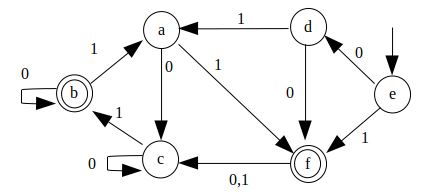
\includegraphics[width=3in]{Capture0.JPG}
\end{center}

\nextq
\tf. $\epsilon$ is accepted by $M$.
\\
\ANSWER
\begin{answerlong}
F
\end{answerlong}

\nextq
\tf. $00$ is accepted by $M$.
\\
\ANSWER
\begin{answerlong}
T
\end{answerlong}

\nextq
\tf. $01$ is accepted by $M$.
\\
\ANSWER
\begin{answerlong}
T
\end{answerlong}

\nextq
\tf. $10$ is accepted by $M$.
\\
\ANSWER
\begin{answerlong}
T
\end{answerlong}

\nextq
\tf. $11$ is accepted by $M$.
\\
\ANSWER
\begin{answerlong}
T
\end{answerlong}

\nextq
\tf. $111000 \in L(M)$.
\\
\ANSWER
\begin{answerlong}
T
\end{answerlong}

%------------------------------------------------------------------------------
The following is NFA $N$:
\begin{center}
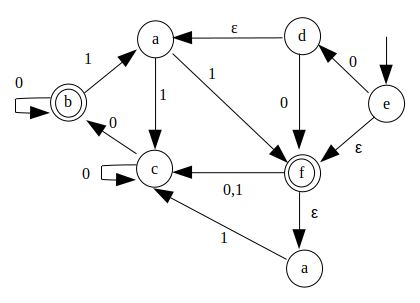
\includegraphics[width=3in]{Capture.JPG}
\end{center}

\nextq
\tf. $\epsilon$ is accepted by $N$.
\\
\ANSWER
\begin{answerlong}
T
\end{answerlong}

\nextq
\tf. $00$ is accepted by $N$.
\\
\ANSWER
\begin{answerlong}
T
\end{answerlong}

\nextq
\tf. $01$ is accepted by $N$.
\\
\ANSWER
\begin{answerlong}
T
\end{answerlong}

\nextq
\tf. $10$ is accepted by $N$.
\\
\ANSWER
\begin{answerlong}
T
\end{answerlong}

\nextq
\tf. $11$ is accepted by $N$.
\\
\ANSWER
\begin{answerlong}
T
\end{answerlong}

\nextq
\tf. $111000 \in L(N)$.
\\
\ANSWER
\begin{answerlong}
T
\end{answerlong}

%------------------------------------------------------------------------------
\newpage

\textsc{Instructions}

In \verb!main.tex! change the email address in
\begin{console}
\renewcommand\AUTHOR{jdoe5@cougars.ccis.edu} 
\end{console}
yours.
In the bash shell, execute \lq\lq \verb!make!" to recompile \verb!main.pdf!.
Execute \lq\lq \verb!make v!" to view \verb!main.pdf!.
Execute \lq\lq \verb!make s!" to create \verb!submit.tar.gz! for submission.

For each question, you'll see boxes for you to fill.
You write your answers in \verb!main.tex! file.
For small boxes, if you see
\begin{console}[frame=single=single,fontsize=\small]
1 + 1 = \answerbox{}.
\end{console}
you do this:
\begin{console}[frame=single=single,fontsize=\small]
1 + 1 = \answerbox{2}.
\end{console}
\verb!answerbox! will also appear in
\lq\lq true/false" and \lq\lq multiple-choice"
questions.

For longer answers that needs typewriter font, if you see
\begin{console}[frame=single=single, fontsize=\small]
Write a C++ statement that declares an integer variable name x.
\begin{answercode}
\end{answercode}
\end{console}
you do this:
\begin{console}[frame=single=single, fontsize=\small]
Write a C++ statement that declares an integer variable name x.
\begin{answercode}
int x;
\end{answercode}
\end{console}
\verb!answercode! will appear in questions asking for
code, algorithm, and program output.
In this case, indentation and spacing is significant.
For program output, I do look at spaces and newlines.

For long answers (not in typewriter font) if you see
\begin{console}[frame=single=single, fontsize=\small]
What is the color of the sky?
\begin{answerlong}
\end{answerlong}
\end{console}
you can write
\begin{console}[frame=single=single, fontsize=\small]
What is the color of the sky?
\begin{answerlong}
The color of the sky is blue.
\end{answerlong}
\end{console}
For students beyond 245: You can put \LaTeX\ commands in
\verb!answerbox! and 
\verb!answerlong!.

A question that begins with \lq\lq T or F or M"
requires you to identify whether it is true or
false, or meaningless.
\lq\lq Meaningless" means something's wrong with the statement and
it is not well-defined.
Something like \lq\lq $1 +_2$" or \lq\lq $\{2\}^{\{3\}}$" is not
well-defined.
Therefore a question such as
\lq\lq Is $42 = 1 +_2$ true or false?" or
\lq\lq Is $42 = \{2\}^{\{3\}}$ true or false?"
does not make sense.
\lq\lq Is $P(42) = \{42\}$ true or false?" is meaningless because $P(X)$
is only defined if $X$ is a set.
For \lq\lq Is 1 + 2 + 3 true or false?", \lq\lq 1 + 2 + 3" is well--defined but
as a
\lq\lq numerical expression", not as a \lq\lq proposition", i.e.,
it cannot be true or false.
Therefore \lq\lq Is 1 + 2 + 3 true or false?" is also not a well-defined
question.

When writing results of computations, make sure it's simplified.
For instance write $2$ instead of $1 + 1$.
When you write down sets,
if the answer is $\{1\}$, I do not
want to see $\{1, 1\}$.

When writing a counterexample, always write the simplest.

Here are some examples (see \verb!instructions.tex! for details):

\begin{enumerate}

 \item \tf: 1 + 1 = 2 \dotfill\answerbox{T}
 
 \item \tf: 1 + 1 = 3 \dotfill\answerbox{F}
 
 \item \tf: $1 +^2 =$ \dotfill\answerbox{M}
 
 \item $1 + 2 =$ \answerbox{3}
 
 \item Write a C++ statement to declare an integer variable named
 \verb!x!.
 \begin{answercode}
int x;
 \end{answercode}

 \item Solve $x^2 - 1 = 0$.
 \begin{answerlong}
 Since $x^2 - 1 = (x-1)(x+1)$, $x^2 - 1 = 0$ implies $(x-1)(x+1)=0$.
 Therefore $x - 1 = 0$ or $x = -1$.
 Hence $x = 1$ or $x = -1$.
 \end{answerlong}

 \item
 \begin{mcq}
 {Which is true?}{\answerbox{C}}
 {$1+1=0$}
 {$1+1=1$}
 {$1+1=2$}
 {$1+1=3$}
 {$1+1=4$}
 \end{mcq}


\end{enumerate}

\end{document}
